%!TEX TS-program = xelatex
%!TEX encoding = UTF-8 Unicode

\documentclass[11pt,tikz,border=1]{standalone}
\usetikzlibrary{decorations.pathreplacing}

\begin{document}
  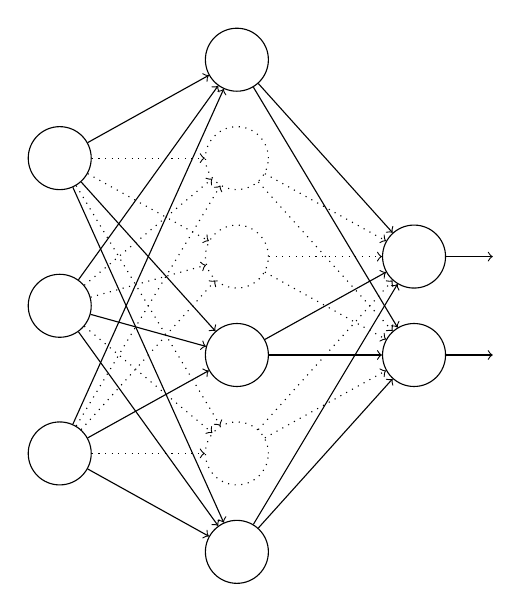
\begin{tikzpicture}[
    neuron/.style={circle,draw,inner sep=0pt,minimum size=8mm}
    ]

    % left layers:
    \foreach \y in {0,...,2}
      \node (l\y) at (0, \y * 1.875 + 2 * 1.25) [neuron] {};

    % middle layers:
    \foreach \y in {0,2,5}
      \node (m\y) at (2.25, \y * 1.25 + 1 * 1.25) [neuron] {};
    
    \foreach \y in {1,3,4}
      \node (m\y) at (2.25, \y * 1.25 + 1 * 1.25) [neuron,dotted] {};

    % right layer:
    \node (r0) at (4.5, 5) [neuron] {};
    \node (r1) at (4.5, 3.75) [neuron] {};

    % connections:
    \foreach \x in {0,...,2}
      \foreach \y in {0,2,5}
        \draw [->] (l\x) to (m\y);

    \foreach \x in {0,...,2}
      \foreach \y in {1,3,4}
        \draw [dotted,->] (l\x) to (m\y);

    \foreach \x in {0,2,5}
      \foreach \y in {0,1}
        \draw [->] (m\x) to (r\y);

    \foreach \x in {1,3,4}
      \foreach \y in {0,1}
        \draw [dotted,->] (m\x) to (r\y);
        
    \draw[->] (r0) -- ++(1,0);
    \draw[->] (r1) -- ++(1,0);

  \end{tikzpicture} 
\end{document}
